\documentclass[8pt]{beamer}

\usetheme{Madrid}
\usecolortheme{crane}
\linespread{1.5}

\usepackage{graphicx}
\usepackage{physics}
\usepackage{hyperref}
\usepackage{slashed}
\usepackage{siunitx}
\usepackage{lmodern}

%\newcommand{\phanitem}{\phantom{\item}}
\newcommand{\lag}{\mathcal{L}}

\title{Standard Model Effective Field Theory}
\author{Yingsheng Huang}
\institute{Institute of High Energy Physics}
\begin{document}
\maketitle
\begin{frame}
  \frametitle{Content}
  \tableofcontents
\end{frame}
\section{Revisit Effective Field Theory}
\begin{frame}
  \frametitle{Revisit EFT}
  Basic idea of effective theory: Low energy approximation of underlying high energy theory.

  Examples:
  \begin{itemize}
    \item Astronomy study
	%\phanitem
    \item Classical electrodynamics
    %\phanitem
	\item Rayleigh scattering
	\item Hydrogen atom spectra
    \item \dots
  \end{itemize}
  Historical review:
  \begin{itemize}
    \item Field-theoretic appearance of current algebra

    From linear $\sigma$ model to direct derivation
    \item Wilson's renormalization group
	\item Applications of EFT in strong interaction
  \end{itemize}
\end{frame}
\begin{frame}
    \frametitle{Basic properties and applications of EFT}
    Power counting:
    $$\lag_I=\sum_{i=0}^{\infty}\frac{g_i}{\Lambda_i}\hat O_i$$
    Accuracy increases with higher $i$.

    Renormalizability: Even if the underlying theory
is renormalizable, once a finite cutoff is introduced it becomes necessary to
introduce every possible interaction, renormalizable or not, to keep physics
strictly cutoff independent. From this point of view, it doesn’t make much
difference whether the underlying theory is renormalizable or not.

	Matching.

    Famous examples:
    \begin{itemize}
      \item Euler-Heisenberg Lagrangian
      \item NRQED
      \item Chiral perturbation theory
    \end{itemize}
\end{frame}
\section{Standard Model Effective Field Theory}
\begin{frame}
  \frametitle{Motivation}
  \begin{itemize}
  \item SM is not the fundermantal theory.

  \item LHC: the last piece of standard model has been found, yet no new physics.

  \item Which directions in the parameter space of ”deformations” of the SM are still
unprobed?

  \item Provide a useful guidance for future experiments.

  \item Provide insight into some of the
many long standing experimental observations that remain unexplained.

  \item Place constraints on specific UV models.

  \item Estimate the physics reach (i.e. the largest $\Lambda$) of specific UV models.
  \end{itemize}

\end{frame}
\begin{frame}
  \frametitle{Standard Model Effective Field Theory}
  A model independent approach of BSM physics.

  Two different ways of BSM: search for new particles, or new interactions of known particles. SMEFT is of the latter.

  Principles of constructing such theory:
  \begin{itemize}
	\item Do not break the framework of SM itself, and respect all axioms of QFT (since it must be a QFT).
	\item Respect $SU(3)_C\cross SU(2)_L\cross U(1)_Y$ gauge symmetry. (Unbroken above Higgs mass.)
	\item Assume that the new interactions decouple from the Standard Model in the limit
that the energy scale that characterizes the new interactions goes to infinity.
	\item Ideally new interaction should
be able to calculate any process at any order in both the Standard Model interactions and
the new interactions.
  \end{itemize}

  Basic idea of SMEFT: Consider Standard Model itself as an effective field theory, and add higher dimensional opeartors to mimic the effect of BSM physics (connect UV models to EW and/or Higgs observables).
\end{frame}
\begin{frame}
  The effective Lagrangian is of the form
  $$\lag=\lag_{SM}+\sum_{i=0}^{\infty}\frac{c_i}{\Lambda_i^2}\hat O_i+\dots$$
  \begin{itemize}
  \item $c_i$ is a dimensionless coefficient. $\hat{O}_i$ is an opeartor of mass dimension six constructed from SM fields. The ellipsis stands for higher mass dimensions.
  \item Energy scale $\Lambda$, interpreted
as the scale of new physics and that we assume to be greater than the Higgs mass.
  \item New
interactions are constructed from Standard Model fields and have a coefficient proportional
to an inverse power of $\Lambda$; thus the Standard Model is recovered in the limit $\Lambda\rightarrow\infty$.
  \item The
new interactions are compatible with the calculation of Standard Model radiative corrections.
The new interactions may be calculated to any desired order in $1/\Lambda$, with the caveat that
the introduction of additional interactions may be necessary at each order in $1/\Lambda$.
  \end{itemize}

\end{frame}
\begin{frame}
  Benefit of such theory:
  \begin{itemize}
	\item The possiblity of SM containing non-renormalizable interactions (have coefficients proportional to inverse power of $\Lambda$) is therefore supressed below $\Lambda$.
	\item Give guidance of the types of new interactions. (e.g. consider dominant term is of $1/\Lambda$ order, only one possible interaction which is the one gives rise to Majorana masses for neutrinos; but to conserve Baryon and Lepton number B \& L, all interactions must proportion to even order of $1/\Lambda$.)
	\item Easier and, in pratical purposes, usually more accurate than the computation of specific UV models (which may involve loop-order).
  \end{itemize}
\end{frame}
\begin{frame}
  \frametitle{An example}
  Consider a new $Z'$ boson coupled to SM fermions.

  At low energy, it's a four fermion interaction.

  Each fermion gives mass dimension of $3/2$, so it's a dimension-six opeartor.

  Similar to the SM Z boson, the vertex is proportional to $\frac{1}{m_{Z'}^2}$, which makes $m_{Z'}$ the energy scale.

  $\Longrightarrow$ An effective field theory is not supposed to be valid at any arbitrarily high energy. In this case it's valid below $m_{Z'}$.

  Beyond that energy, the new $Z'$ particle must be included explicitly.

  Note that in this example, we can also see that measuring the coefficient $\frac{c_i}{\Lambda_i}$ wouldn't give the energy scale $\Lambda$, it only gives the overall coupling $G_F'$.
\end{frame}
\begin{frame}
  \frametitle{Construction of dimension-six opeartors}
  First we study the dimension-five terms (and why only the neutrino mass and mixing part survived).

  Applying gauge symmetry of SM, only one possiblity survived.
  $$Q_{vv}=\epsilon_{jk}\epsilon_{mn}\varphi^j\varphi^m(l^k_p)^TCl^n_r=(\tilde\varphi^{\dagger}l_p)^TC(\tilde \varphi^{\dagger}l_r)$$
  where $\tilde \varphi^j=\epsilon_{jk}(\varphi^k)^*$, $C$ is the charge conjugate matrix. Clearly it's a dimension-five opeartor, after SSB it provides neutrino Majorana masses and mixing.

  For dimension-six opeartors, they can be divide into CP-odd part (all terms containing $\tilde G$ and such) and CP-even part. Applying gauge symmetry and EOM, all possible terms are listed in the following tables.

  Experiment constrains: $B$ $L$ conservation, $D=6$ terms relatively small, only $CP$ even part for tree level, etc.

  %Example: the $\varphi^2D^4$ operator. 

 % Only consider derivatives act on one $\varphi$, ignore $\epsilon^{\mu\nu\rho\sigma}$ terms, 


\end{frame}
\begin{frame}
  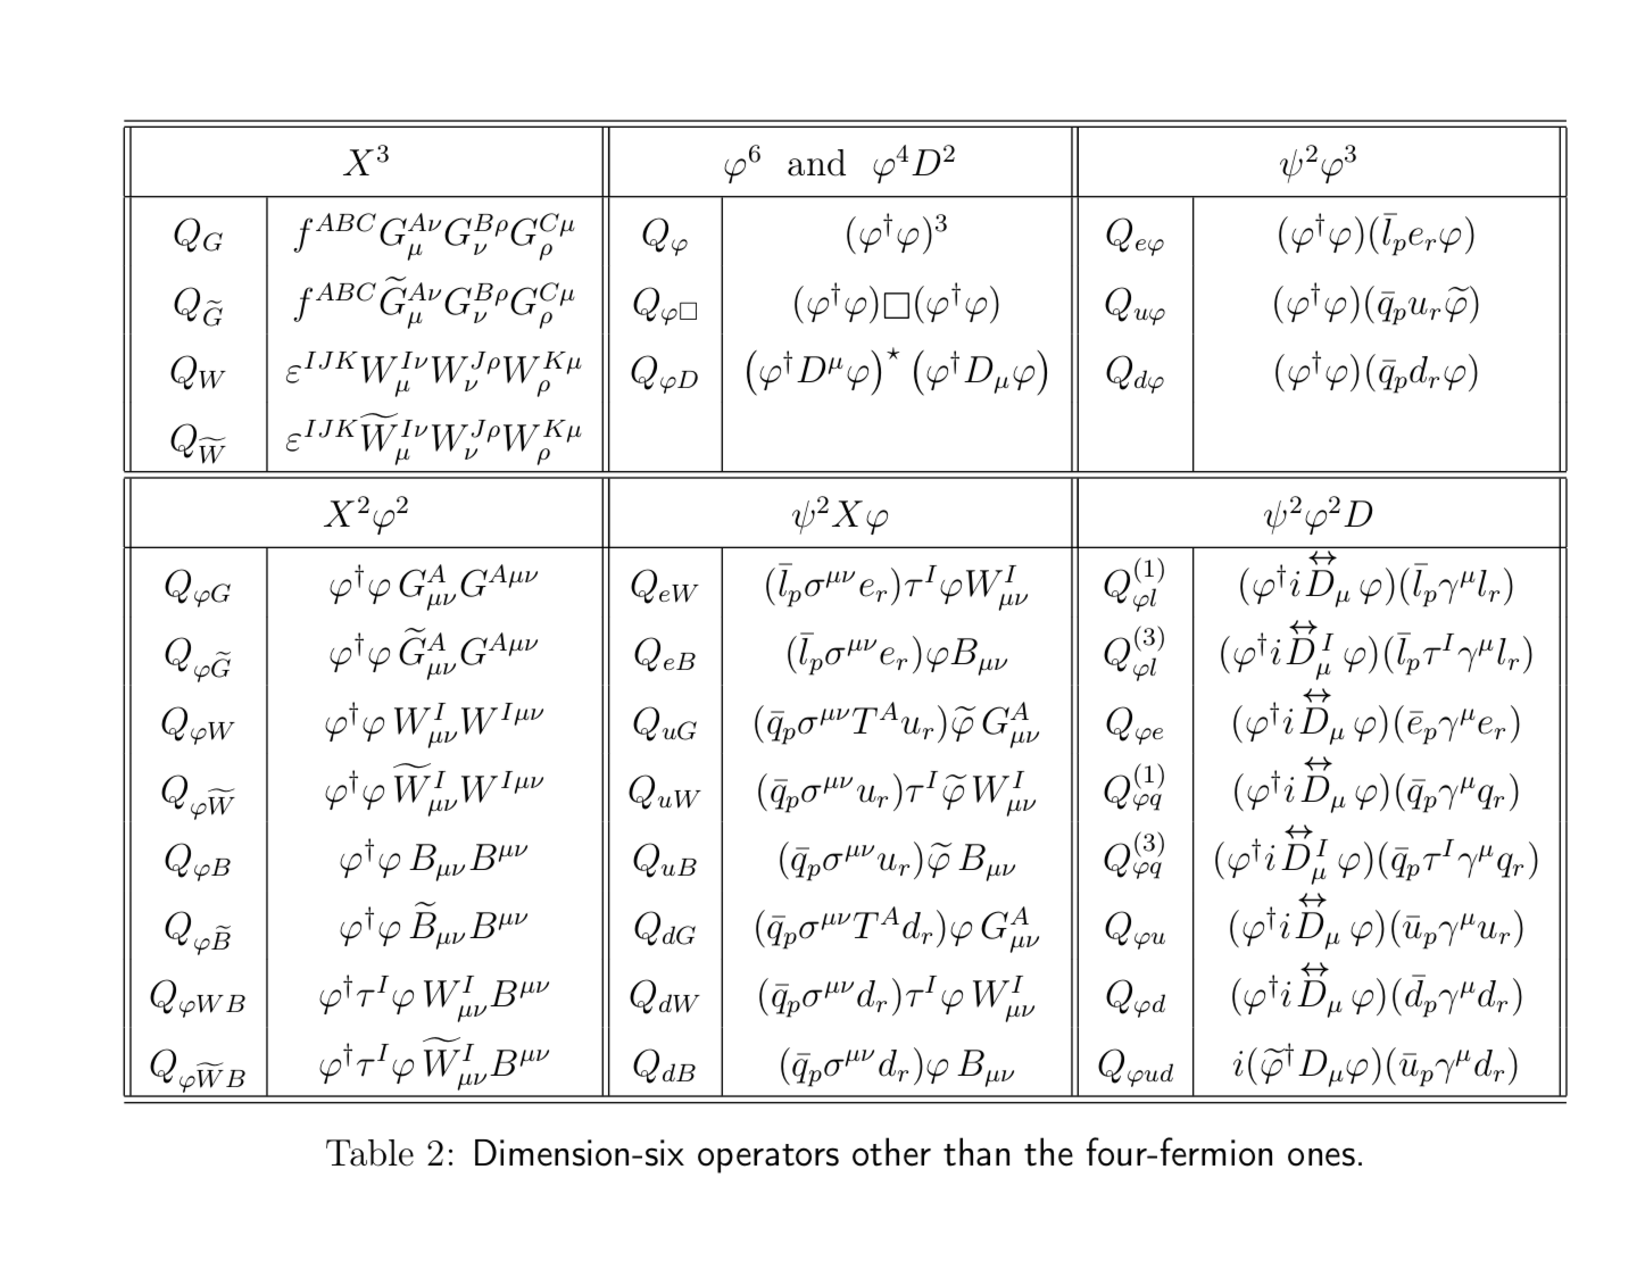
\includegraphics[width=5in]{boson.pdf}
\end{frame}
\begin{frame}
  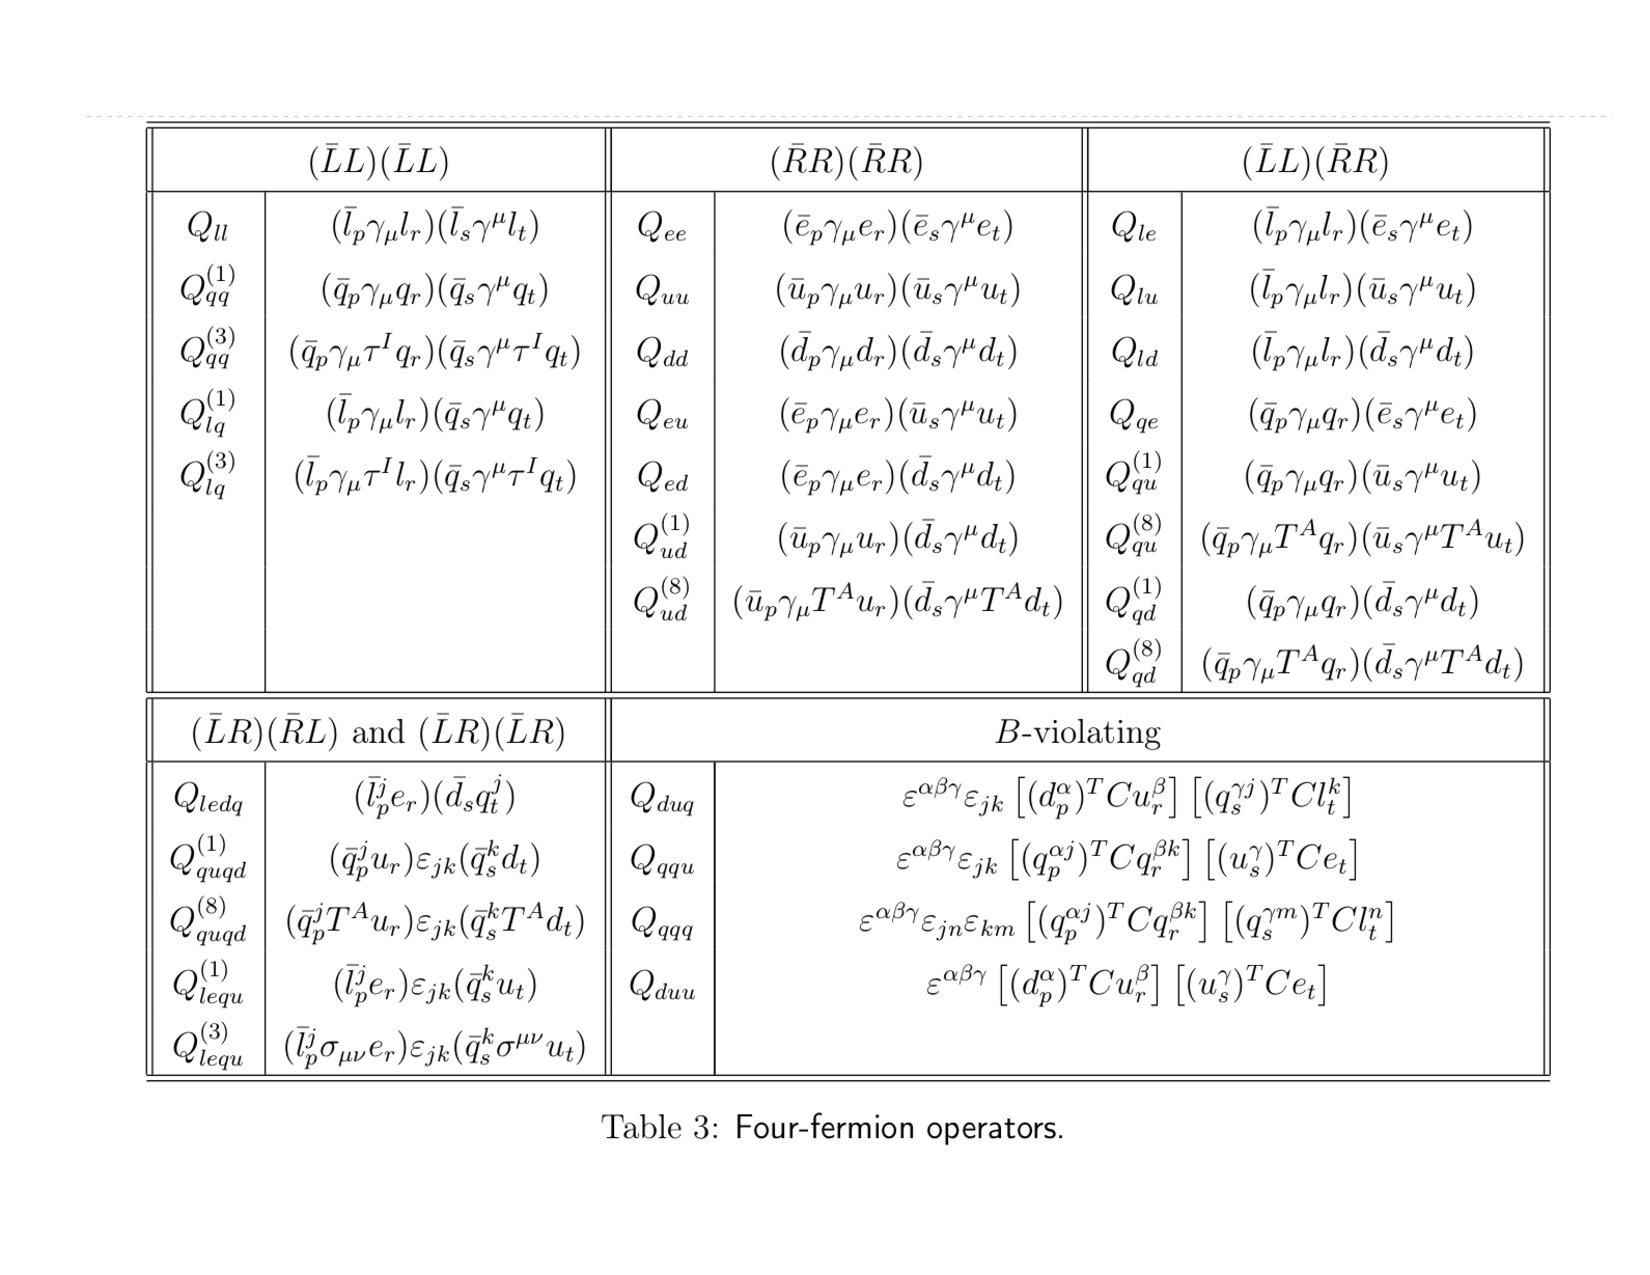
\includegraphics[width=5in]{fermion.pdf}
\end{frame}
%\begin{frame}
%  $X^3$ terms: 
%\end{frame}
\begin{frame}
   \frametitle{How to use SMEFT?}
   The procedure for any EFT:
   \begin{enumerate}
     \item Matching: matching some UV models onto the EFT at $\Lambda$ scale
     \item Running: running the coupling to weak scale, using RG equation for EFT
     \item Mapping: mapping the Wilson coefficients onto observables
   \end{enumerate}
   Convenient way of matching process: covariant derivative expansion (CDE)

   When to choose an opeartor basis?

   In matching stage, one should integrate out the massive modes and obtain the effective actions which contains higher-dimension operators.

   In the running stage, one can choose the UV-obtained basis or switch to other ones.

   After having the parameterized obserables, we can compare it with experimental values, which gives some constrains on parameters.
\end{frame}
\section{Summary}
\begin{frame}
  \frametitle{Summary}
  \begin{itemize}
  \item SMEFT is an efficient and systematic way of mimicing the effect of new physics. 
  
  \item The idea is to take SM as an effective theory where the renormalizable SM might just be the first term of the whole theory.

  \item The constrains of SMEFT are only some given symmetry requests, Lorentz invariance and the basic property of field theory.
  
  \item By integrating out the heavy particles, the effecitve Lagrangian is obtained. With RG equation, we can have EW and Higgs observables at any scale lower than the effecitve limit.
  \end{itemize}
\end{frame}
\begin{frame}
    \frametitle{Reference}
    \begin{thebibliography}{b}
    \footnotesize
	\bibitem{Weinberg:2016kyd}
	  S.~Weinberg,
	  %``Effective field theory, past and future,''
	  Int.\ J.\ Mod.\ Phys.\ A {\bf 31}, no. 06, 1630007 (2016).
	  doi:10.1142/S0217751X16300076
	  %%CITATION = doi:10.1142/S0217751X16300076;%%
	  %1 citations counted in INSPIRE as of 17 Jun 2017
	\bibitem{Holstein:2000ap}
	  B.~R.~Holstein,
	  %``Introduction to effective field theory,''
	  Nucl.\ Phys.\ A {\bf 689}, 135 (2001)
	  doi:10.1016/S0375-9474(01)00828-4
	  [nucl-th/0010015].
	  %%CITATION = doi:10.1016/S0375-9474(01)00828-4;%%
	  %7 citations counted in INSPIRE as of 18 Jun 2017
	\bibitem{Burgess:2007pt}
	  C.~P.~Burgess,
	  %``Introduction to Effective Field Theory,''
	  Ann.\ Rev.\ Nucl.\ Part.\ Sci.\  {\bf 57}, 329 (2007)
	  doi:10.1146/annurev.nucl.56.080805.140508
	  [hep-th/0701053].
	  %%CITATION = doi:10.1146/annurev.nucl.56.080805.140508;%%
	  %134 citations counted in INSPIRE as of 18 Jun 2017
	\bibitem{Pomarol:2013zra}
	  A.~Pomarol and F.~Riva,
	  %``Towards the Ultimate SM Fit to Close in on Higgs Physics,''
	  JHEP {\bf 1401}, 151 (2014)
	  doi:10.1007/JHEP01(2014)151
	  [arXiv:1308.2803 [hep-ph]].
	  %%CITATION = doi:10.1007/JHEP01(2014)151;%%
	  %148 citations counted in INSPIRE as of 18 Jun 2017
	\bibitem{Willenbrock:2014bja}
	S.~Willenbrock and C.~Zhang,
	  %``Effective Field Theory Beyond the Standard Model,''
	  Ann.\ Rev.\ Nucl.\ Part.\ Sci.\  {\bf 64}, 83 (2014)
	  doi:10.1146/annurev-nucl-102313-025623
	 [arXiv:1401.0470 [hep-ph]].
	  %%CITATION = doi:10.1146/annurev-nucl-102313-025623;%%
	 %41 citations counted in INSPIRE as of 18 Jun 2017
	 \bibitem{Grzadkowski:2010es} 
	  B.~Grzadkowski, M.~Iskrzynski, M.~Misiak and J.~Rosiek,
	  %``Dimension-Six Terms in the Standard Model Lagrangian,''
	  JHEP {\bf 1010}, 085 (2010)
	  doi:10.1007/JHEP10(2010)085
	  [arXiv:1008.4884 [hep-ph]].
	  %%CITATION = doi:10.1007/JHEP10(2010)085;%%
	  %559 citations counted in INSPIRE as of 20 Jun 2017
	 \bibitem{Henning:2014wua}
	 B.~Henning, X.~Lu and H.~Murayama,
	  %``How to use the Standard Model effective field theory,''
	  JHEP {\bf 1601}, 023 (2016)
	  doi:10.1007/JHEP01(2016)023
	  [arXiv:1412.1837 [hep-ph]].
	  %%CITATION = doi:10.1007/JHEP01(2016)023;%%
	  %78 citations counted in INSPIRE as of 19 Jun 2017

    \end{thebibliography}
\end{frame}
\end{document}
